\documentclass[]{beamer}\makeatletter

\IfFileExists{xcolor.sty}%
  {\RequirePackage{xcolor}}%
  {\RequirePackage{color}}
\usepackage{colortbl}
\usepackage{wrapfig}
\usepackage{ifxetex}
\ifxetex
  \usepackage{fontspec}
  \usepackage{xunicode}
  \catcode`⃥=\active \def⃥{\textbackslash}
  \catcode`❴=\active \def❴{\{}
  \catcode`❵=\active \def❵{\}}
  \def\textJapanese{\fontspec{Kochi Mincho}}
  \def\textChinese{\fontspec{HAN NOM A}\XeTeXlinebreaklocale "zh"\XeTeXlinebreakskip = 0pt plus 1pt }
  \def\textKorean{\fontspec{Baekmuk Gulim} }
  \setmonofont{DejaVu Sans Mono}
  
\else
  \IfFileExists{utf8x.def}%
   {\usepackage[utf8x]{inputenc}
      \PrerenderUnicode{–}
    }%
   {\usepackage[utf8]{inputenc}}
  \usepackage[english]{babel}
  \usepackage[T1]{fontenc}
  \usepackage{float}
  \usepackage[]{ucs}
  \uc@dclc{8421}{default}{\textbackslash }
  \uc@dclc{10100}{default}{\{}
  \uc@dclc{10101}{default}{\}}
  \uc@dclc{8491}{default}{\AA{}}
  \uc@dclc{8239}{default}{\,}
  \uc@dclc{20154}{default}{ }
  \uc@dclc{10148}{default}{>}
  \def\textschwa{\rotatebox{-90}{e}}
  \def\textJapanese{}
  \def\textChinese{}
  \IfFileExists{tipa.sty}{\usepackage{tipa}}{}
  \usepackage{times}
\fi
\def\exampleFont{\ttfamily\small}
\DeclareTextSymbol{\textpi}{OML}{25}
\usepackage{relsize}
\RequirePackage{array}
\def\@testpach{\@chclass
 \ifnum \@lastchclass=6 \@ne \@chnum \@ne \else
  \ifnum \@lastchclass=7 5 \else
   \ifnum \@lastchclass=8 \tw@ \else
    \ifnum \@lastchclass=9 \thr@@
   \else \z@
   \ifnum \@lastchclass = 10 \else
   \edef\@nextchar{\expandafter\string\@nextchar}%
   \@chnum
   \if \@nextchar c\z@ \else
    \if \@nextchar l\@ne \else
     \if \@nextchar r\tw@ \else
   \z@ \@chclass
   \if\@nextchar |\@ne \else
    \if \@nextchar !6 \else
     \if \@nextchar @7 \else
      \if \@nextchar (8 \else
       \if \@nextchar )9 \else
  10
  \@chnum
  \if \@nextchar m\thr@@\else
   \if \@nextchar p4 \else
    \if \@nextchar b5 \else
   \z@ \@chclass \z@ \@preamerr \z@ \fi \fi \fi \fi
   \fi \fi  \fi  \fi  \fi  \fi  \fi \fi \fi \fi \fi \fi}
\gdef\arraybackslash{\let\\=\@arraycr}
\def\@textsubscript#1{{\m@th\ensuremath{_{\mbox{\fontsize\sf@size\z@#1}}}}}
\def\Panel#1#2#3#4{\multicolumn{#3}{){\columncolor{#2}}#4}{#1}}
\def\abbr{}
\def\corr{}
\def\expan{}
\def\gap{}
\def\orig{}
\def\reg{}
\def\ref{}
\def\sic{}
\def\persName{}\def\name{}
\def\placeName{}
\def\orgName{}
\def\textcal#1{{\fontspec{Lucida Calligraphy}#1}}
\def\textgothic#1{{\fontspec{Lucida Blackletter}#1}}
\def\textlarge#1{{\large #1}}
\def\textoverbar#1{\ensuremath{\overline{#1}}}
\def\textquoted#1{‘#1’}
\def\textsmall#1{{\small #1}}
\def\textsubscript#1{\@textsubscript{\selectfont#1}}
\def\textxi{\ensuremath{\xi}}
\def\titlem{\itshape}
\newenvironment{biblfree}{}{\ifvmode\par\fi }
\newenvironment{bibl}{}{}
\newenvironment{byline}{\vskip6pt\itshape\fontsize{16pt}{18pt}\selectfont}{\par }
\newenvironment{citbibl}{}{\ifvmode\par\fi }
\newenvironment{docAuthor}{\ifvmode\vskip4pt\fontsize{16pt}{18pt}\selectfont\fi\itshape}{\ifvmode\par\fi }
\newenvironment{docDate}{}{\ifvmode\par\fi }
\newenvironment{docImprint}{\vskip 6pt}{\ifvmode\par\fi }
\newenvironment{docTitle}{\vskip6pt\bfseries\fontsize{18pt}{22pt}\selectfont}{\par }
\newenvironment{msHead}{\vskip 6pt}{\par}
\newenvironment{msItem}{\vskip 6pt}{\par}
\newenvironment{rubric}{}{}
\newenvironment{titlePart}{}{\par }

\newcolumntype{L}[1]{){\raggedright\arraybackslash}p{#1}}
\newcolumntype{C}[1]{){\centering\arraybackslash}p{#1}}
\newcolumntype{R}[1]{){\raggedleft\arraybackslash}p{#1}}
\newcolumntype{P}[1]{){\arraybackslash}p{#1}}
\newcolumntype{B}[1]{){\arraybackslash}b{#1}}
\newcolumntype{M}[1]{){\arraybackslash}m{#1}}
\definecolor{label}{gray}{0.75}
\def\unusedattribute#1{\sout{\textcolor{label}{#1}}}
\DeclareRobustCommand*{\xref}{\hyper@normalise\xref@}
\def\xref@#1#2{\hyper@linkurl{#2}{#1}}
\begingroup
\catcode`\_=\active
\gdef_#1{\ensuremath{\sb{\mathrm{#1}}}}
\endgroup
\mathcode`\_=\string"8000
\catcode`\_=12\relax

\usepackage{framed}
\definecolor{shadecolor}{gray}{0.95}
\usepackage{colortbl}
\usepackage{longtable}
\usepackage[normalem]{ulem}
\usetheme{PaloAlto}
\usepackage{times}
\usepackage{fancyvrb}
\usepackage{fancyhdr}
\def\Gin@extensions{.pdf,.png,.jpg,.mps,.tif}
\xdefinecolor{blue1}{rgb}{0, 0, 0.7}
\xdefinecolor{blue2}{rgb}{0, 0, 1}
\setbeamercovered{transparent}
\let\mainmatter\relax
\let\frontmatter\relax
\let\backmatter\relax
\let\endfoot\relax
\let\endlastfoot\relax

  \usepackage{endnotes}
  
      \def\theendnote{\@alph\c@endnote}
    
\date{}
\institute{}
\def\TheFullDate{1970-01-01}
\def\TheID{\makeatother }
\def\TheDate{1970-01-01}
\title{Test 6}
\author{}\makeatletter \makeatother 
\begin{document}

     \frame{\maketitle}
   \let\tabcellsep& 
  \begin{frame} 
  \frametitle{Outline} 
  \tableofcontents
  \end{frame}

\begin{frame}
\frametitle{Part 1}\par
\textcolor{red}{Cats}\footnote{A Cat (\url{http://en.wikipedia.org/wiki/Cat}) is a fine beast, as in this picture: 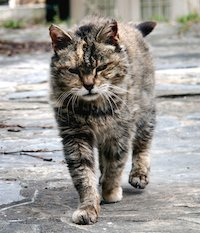
\includegraphics[width=\textwidth]{cat.jpg}}
\end{frame}

\begin{frame}
\frametitle{Part 2}\par
Dogs\endnote{A Dog (\url{http://en.wikipedia.org/wiki/Dog}) is a dreary beast, unlike the cat in this picture: 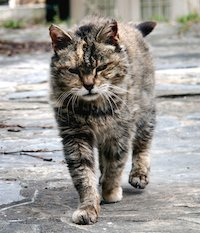
\includegraphics[width=\textwidth]{cat.jpg}}
\end{frame}

\begin{frame}
\frametitle{cit and quote}\par

\begin{quote}
 \par
Ils ne produisent qu’en collaborant d’une manière déterminée et en échangeant entre eux leurs activités. Pour produire, ils entrent en relations et en rapports déterminés les uns avec les autres, et ce n’est que dans les limites de ces relations et de ces rapports sociaux que s’établit leur action sur la nature, la production.\par
\begin{biblfree} Karl Marx, \textit{Travail salarié et capital, suivi de Salaire, prix et profit}, p. 31, Éditions sociales, Paris, 1952.\end{biblfree}
\end{quote}
\par
Some text introducing \textit{all things bibliographic}, followed by some more text.
\end{frame}

\begin{frame}[fragile]
\frametitle{Verbatim}
\bgroup\ttfamily\fontsize{8.5pt}{9pt}\selectfont\par
\begin{exampleblock}{}
\noindent\ttfamily\mbox{}{\color{blue1}<\textbf{xsl:template}\hspace*{4pt}{\color{blue2}name}="{\color{blue2}makeExternalLink}"\mbox{}\newline 
   xmlns:xsl="http://www.w3.org/1999/XSL/Transform">}\mbox{}\newline 
\hspace*{4pt}{\color{blue1}<\textbf{xsl:param}\hspace*{4pt}{\color{blue2}name}="{\color{blue2}ptr}"\hspace*{4pt}{\color{blue2}as}="{\color{blue2}xs:boolean}"\mbox{}\newline 
\hspace*{4pt}\hspace*{4pt}{\color{blue2}select}="{\color{blue2}false()}"/>}\mbox{}\newline 
\hspace*{4pt}{\color{blue1}<\textbf{xsl:param}\hspace*{4pt}{\color{blue2}name}="{\color{blue2}dest}"/>}\mbox{}\newline 
\hspace*{4pt}{\color{blue1}<\textbf{xsl:choose}>}\mbox{}\newline 
\hspace*{4pt}\hspace*{4pt}{\color{blue1}<\textbf{xsl:when}\hspace*{4pt}{\color{blue2}test}="{\color{blue2}\$ptr}">}\mbox{}\newline 
\hspace*{4pt}\hspace*{4pt}\hspace*{4pt}{\color{blue1}<\textbf{xsl:text}>}❴⃥small⃥ttfamily {\color{blue1}</\textbf{xsl:text}>}\mbox{}\newline 
\hspace*{4pt}\hspace*{4pt}\hspace*{4pt}{\color{blue1}<\textbf{xsl:sequence}\hspace*{4pt}{\color{blue2}select}="{\color{blue2}\$dest}"/>}\mbox{}\newline 
\hspace*{4pt}\hspace*{4pt}\hspace*{4pt}{\color{blue1}<\textbf{xsl:text}>}❵{\color{blue1}</\textbf{xsl:text}>}\mbox{}\newline 
\hspace*{4pt}\hspace*{4pt}{\color{blue1}</\textbf{xsl:when}>}\mbox{}\newline 
\hspace*{4pt}\hspace*{4pt}{\color{blue1}<\textbf{xsl:otherwise}>}\mbox{}\newline 
\hspace*{4pt}\hspace*{4pt}\hspace*{4pt}{\color{blue1}<\textbf{xsl:apply-templates}/>}\mbox{}\newline 
\hspace*{4pt}\hspace*{4pt}{\color{blue1}</\textbf{xsl:otherwise}>}\mbox{}\newline 
\hspace*{4pt}{\color{blue1}</\textbf{xsl:choose}>}\mbox{}\newline 
{\color{blue1}</\textbf{xsl:template}>}\mbox{}\newline 
{\color{blue1}<\textbf{xsl:template}\hspace*{4pt}{\color{blue2}name}="{\color{blue2}tableHline}">}\mbox{}\newline 
\hspace*{4pt}{\color{blue1}<\textbf{xsl:text}>}⃥hline {\color{blue1}</\textbf{xsl:text}>}\mbox{}\newline 
{\color{blue1}</\textbf{xsl:template}>}
\end{exampleblock}
\par\egroup
  
\end{frame}

\begin{frame}
\frametitle{Lists}\begin{description}

\item[{[label here]}]item here
\end{description} 
\end{frame}

\theendnotes
\end{document}
